\documentclass{article}

\usepackage[UTF8]{ctex}
\usepackage{amsmath,amssymb}
\usepackage{geometry}
\usepackage{graphicx}
\usepackage{float}

\geometry{a4paper, margin=2.5cm}

\begin{document}

% ============================================================
\section*{Actor-Critic 与 A2C}

\subsection*{先讲一个故事}

你在学钢琴。你的老师有两种教法：

\textbf{教法一（REINFORCE）}：弹完整首曲子，老师在最后评分——「总体 85 分」。
这个信号能告诉你哪个音弹错了吗？不能。
第 3 小节那个跑偏的和弦、第 12 小节的速度失控，全部淹没在「85 分」这一个数字里。
回去你只能靠猜测去改进。

\textbf{教法二（Actor-Critic）}：老师坐在旁边，每弹几个音就给一句评价——「这里太快」「这个和弦不对」「这段处理得很好」。
即时反馈、精准定位，进步快得多。

但问题来了：如果老师在你弹了三个音之后，就认定「我已经摸透这个学生的水平了」，
从此不再认真听，只是机械地说「还可以」……
从那一刻起，你的练习就失去了有效反馈，进步彻底停止。

\textbf{这就是朴素 Actor-Critic 失败的本质}——不是方向错了，而是 Critic 学得太「快」，把一个\underline{很差的策略}的价值函数拟合到几乎完美，导致优势信号归零，Actor 的梯度消失。

本章要解决的核心问题：\textbf{如何让 Critic 的学习速度始终与 Actor 的改进速度保持匹配？}

\subsection*{从 REINFORCE 到 Actor-Critic：为什么要替换回报}

REINFORCE 的策略梯度估计量：

\[
\nabla_\theta J(\theta) = \mathbb{E}_{\tau \sim \pi_\theta}\!\left[\,\sum_{t=0}^{T}
\nabla_\theta \log \pi_\theta(a_t \mid s_t) \cdot G_t\,\right]
\]

其中 $G_t = \sum_{k=t}^{T} \gamma^{k-t} r_k$ 是第 $t$ 步到回合结束的折扣累积奖励（Monte Carlo 回报）。

\textbf{高方差的来源}：$G_t$ 依赖于 $t$ 时刻之后所有未来步骤的随机动作与随机奖励。
回合越长，$G_t$ 的随机性越大，梯度估计的方差越高——靠「整首曲子最终得分」判断「第 3 小节第 2 拍指法对不对」，信噪比极低。

\textbf{核心替换}：用值函数 $V^\pi(s)$ 提供一个基准（baseline），把 $G_t$ 替换为「比平均水平高多少」：

\[
\boxed{G_t \;\longrightarrow\; A^\pi(s_t, a_t) = Q^\pi(s_t, a_t) - V^\pi(s_t)}
\]

这就是\textbf{优势函数（Advantage Function）}。
$A > 0$ 代表「这个动作比平均更好」；$A < 0$ 代表「比平均更差」。
用 $A$ 代替 $G_t$ 的两个好处：（1）减去了与动作无关的基准 $V$，方差降低；（2）只衡量相对好坏，信号更精准。

% ============================================================
\section*{优势函数与 TD 误差}

\subsection*{数学形式化}

设智能体当前策略为 $\pi_\theta$，参数化价值函数为 $V_\phi(s)$。定义：

\begin{itemize}
  \item \textbf{状态价值函数}：$V^\pi(s) = \mathbb{E}_\pi\!\left[\sum_{k=0}^{\infty} \gamma^k r_{t+k} \,\Big|\, s_t=s\right]$
  \item \textbf{动作价值函数}：$Q^\pi(s,a) = \mathbb{E}_\pi\!\left[\sum_{k=0}^{\infty} \gamma^k r_{t+k} \,\Big|\, s_t=s,\,a_t=a\right]$
  \item \textbf{优势函数}：$A^\pi(s,a) = Q^\pi(s,a) - V^\pi(s)$
\end{itemize}

注意 $\mathbb{E}_{a \sim \pi}\!\left[A^\pi(s,a)\right] = 0$——优势函数的期望恒为零，这是它的归一化性质，
保证「好动作」和「坏动作」正好对称分布在零两侧。

\subsection*{单步 TD 误差作为优势的近似}

计算真实的 $Q^\pi(s,a)$ 需要完整的未来奖励序列。可行的近似：

\[
Q^\pi(s_t, a_t) \approx r_t + \gamma V^\pi(s_{t+1}) \quad \text{（单步 bootstrap）}
\]

代入优势函数定义，得到\textbf{单步 TD 误差}（Temporal Difference error）：

\[
\boxed{\delta_t = r_t + \gamma V_\phi(s_{t+1}) - V_\phi(s_t)}
\]

\textbf{翻译成人话}：$\delta_t$ 是「实际拿到的奖励 + 对未来的新预期」比「出发前的旧预期」多还是少。
多 $\Rightarrow$ 这步动作比预期好（正优势）；少 $\Rightarrow$ 比预期差（负优势）。

\textbf{偏差的来源}：$\delta_t$ 用近似值函数 $V_\phi$ 替代了真实 $V^\pi$，引入了函数逼近误差（偏差）。
这是与 Monte Carlo 的本质权衡：\textbf{方差下降，但不再无偏}。

% ============================================================
\section*{朴素 Actor-Critic 为什么失败}

\subsection*{四个故障模式}

最直接的实现：把 REINFORCE 的每回合更新改成每步在线更新，用 $\delta_t$ 代替 $G_t$。
这个想法正确，但有四个潜伏的致命问题：

\begin{enumerate}
  \item \textbf{Fault 1 —— 单步 TD 优势，方差仍然偏高}\\
        $\delta_t$ 只看一步，受随机奖励和 $V_\phi$ 估计误差的双重噪声影响。
        当 $V_\phi$ 尚未收敛时，$\delta_t$ 的估计极不稳定，Actor 梯度信号噪声大。

  \item \textbf{Fault 2 —— 两时间尺度条件被违反}\\
        Konda \& Tsitsiklis（2003）证明：Actor-Critic 的收敛性要求 Critic 的学习率
        $\alpha_w$ 远大于 Actor 的学习率 $\alpha_\theta$，即 $\alpha_\theta / \alpha_w \to 0$。
        朴素实现两者使用相同学习率，使得 Actor 在 Critic 尚未收敛时就开始更新，
        用错误的 $V_\phi$ 计算梯度方向。

  \item \textbf{Fault 3 —— 无熵正则化，策略提前坍缩}\\
        没有熵 bonus，Actor 会迅速把概率堆在某个次优动作上，变为近确定性策略。
        此后即使 $\delta_t$ 偶尔非零，动作分布没有随机性，策略梯度也无法推动探索。

  \item \textbf{Fault 4 —— 无梯度裁剪，参数可能爆炸}\\
        单步 $|\delta_t|$ 有时极大（初始化差的 $V_\phi$），造成巨大参数更新，使网络进入不可恢复的坏区域。
\end{enumerate}

\subsection*{坍缩机制：优势归零 $\Rightarrow$ Actor 冻结}

Fault 3 触发后，四个故障耦合形成自我强化的恶性循环：

\[
\text{无熵} \;\Rightarrow\; \pi \text{ 快速确定化}
\;\Rightarrow\; \text{每个 episode 退化为完全相同的短轨迹}
\]
\[
\Rightarrow\; V_\phi \text{ 迅速拟合这些轨迹（} \delta_t \approx 0 \text{）}
\;\Rightarrow\; \nabla_\theta J \approx 0 \;\Rightarrow\; \text{Actor 永远冻结。}
\]

这是一个\textbf{稳定但灾难性的固定点}：Critic 越「完美」，Actor 越没有改进动力；
Actor 越不动，Critic 就越稳固。系统自我锁死，且这个锁死状态对所有随机种子几乎一致。

\subsection*{实验证据}

图~\ref{fig:naive} 展示了 5 个随机种子下朴素 Actor-Critic 在 CartPole-v1 上的表现：
episode return 从第 $\sim 20$ 轮起彻底钉死在 $\approx 9$（CartPole-v1 最大为 500），500 轮训练毫无进展。
5 条曲线几乎重叠，说明这不是随机性问题，而是 5 个 seed 全部落入了同一个坏固定点。

\begin{figure}[H]
  \centering
  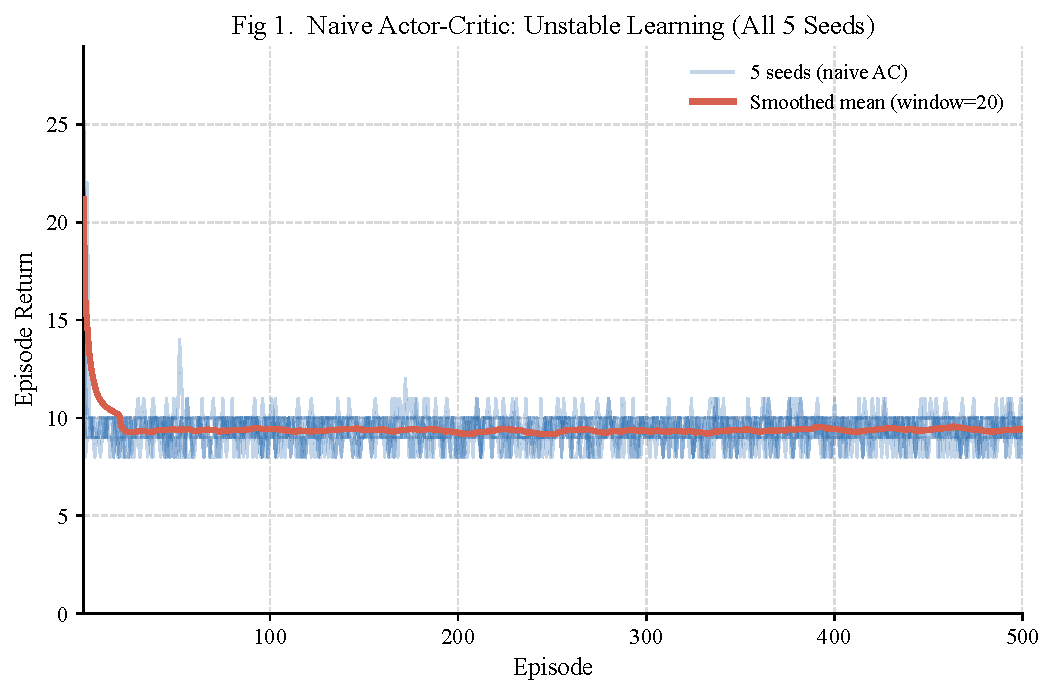
\includegraphics[width=\textwidth]{fig1_naive_ac_failure.pdf}
  \caption{朴素 Actor-Critic（$\alpha = 5 \times 10^{-3}$，无熵，无梯度裁剪）在 CartPole-v1 上的 5 个随机种子：episode return 全程钉死在 $\approx 9$，CartPole-v1 最大回报为 500。}
  \label{fig:naive}
\end{figure}

图~\ref{fig:adv} 给出了坍缩机制的直接证据：朴素 AC 的均值 $|\text{advantage}|$ 在前 50 轮内从 $\approx 3.5$ 急速跌至 $\approx 0.1$，此后全程贴近零轴，Actor 梯度信号彻底消失。
与之对比，A2C 的 $|\text{advantage}|$ 呈现\textbf{钟形曲线}——随策略改进而持续上升（Critic 追不上），随接近收敛而平滑回落——这是在线学习系统的健康特征。

\begin{figure}[H]
  \centering
  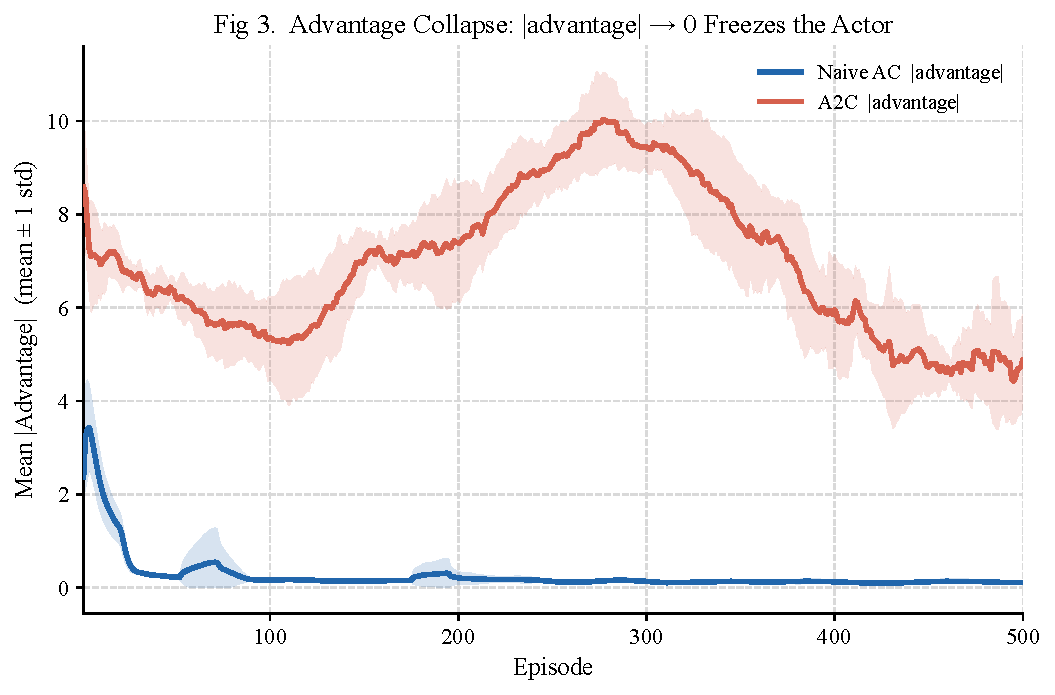
\includegraphics[width=\textwidth]{fig3_advantage_collapse.pdf}
  \caption{每回合均值 $|\hat{A}_t|$ 的演化（5 seeds，mean $\pm$ 1 std）。蓝色（朴素 AC）在前 50 轮内归零；红色（A2C）维持非零信号，钟形轮廓反映了 Critic 与 Actor 之间持续的「追赶」动态。}
  \label{fig:adv}
\end{figure}

% ============================================================
\section*{广义优势估计（GAE）}

\subsection*{偏差--方差权衡的数学框架}

单步 TD 误差 $\delta_t$ 偏差高（$V_\phi$ 不准时）；Monte Carlo 回报 $G_t - V(s_t)$ 方差高（轨迹越长随机性越大）。能不能在两者之间找到可调的中间点？

Schulman et al.\ (2015) 提出\textbf{广义优势估计（Generalized Advantage Estimation, GAE）}：

\[
\boxed{\hat{A}_t^{\,\text{GAE}(\gamma,\lambda)} = \sum_{l=0}^{\infty} (\gamma\lambda)^l \,\delta_{t+l}}
\]

其中每一项 $\delta_{t+l} = r_{t+l} + \gamma V(s_{t+l+1}) - V(s_{t+l})$ 是第 $t+l$ 步的 TD 误差，$\lambda \in [0,1]$ 是插值参数。

\subsection*{推导：GAE 是 TD 误差的几何级数}

展开 GAE 前 $n$ 步：

\[
\hat{A}_t^{(n)} = \sum_{l=0}^{n-1} (\gamma\lambda)^l \delta_{t+l}
= \delta_t + \gamma\lambda\,\delta_{t+1} + (\gamma\lambda)^2 \delta_{t+2} + \cdots
\]

两个极端：

\begin{itemize}
  \item $\lambda = 0$：$\hat{A}_t = \delta_t$（单步 TD），\textbf{高偏差、低方差}，完全依赖 $V_\phi$ 的准确性；
  \item $\lambda = 1$：$(\gamma\lambda)^l = \gamma^l$，对所有未来 TD 误差求和，级数通过望远镜求和（telescoping）等价于
\end{itemize}

\[
\hat{A}_t^{\lambda=1} = \sum_{l=0}^{T-t-1}\gamma^l \delta_{t+l}
= \underbrace{\sum_{l=0}^{T-t-1}\gamma^l r_{t+l}}_{G_t} - V(s_t) + \gamma^{T-t}V(s_T)
\approx G_t - V(s_t), \quad \text{（终态 }V(s_T)\approx 0\text{）}
\]

即退化为 REINFORCE 的 baseline 优势，\textbf{低偏差、高方差}。

\[
\begin{array}{c|c|c}
\lambda & \text{极端情形} & \text{偏差 / 方差} \\
\hline
0 & \hat{A}_t = \delta_t \;\text{（单步 TD）} & \text{高偏差，低方差} \\
1 & \hat{A}_t = G_t - V(s_t) \;\text{（Monte Carlo）} & \text{低偏差，高方差} \\
\lambda \in (0,1) & \text{几何插值} & \text{可控权衡} \\
\end{array}
\]

\textbf{为什么几何衰减合理？} 近期 TD 误差信噪比更高（$V_\phi$ 对近期状态预测更准），远期 TD 误差累积了更多随机性。用 $(\gamma\lambda)^l$ 赋予近期更大权重，相当于对梯度估计做了隐式的指数平滑。

\subsection*{GAE 的实际使用}

GAE 计算需要完整的 TD 误差序列，因此要先完成一整局 rollout，再从末态向前递推：

\[
\hat{A}_{T-1} = \delta_{T-1}, \qquad
\hat{A}_t = \delta_t + \gamma\lambda\,\hat{A}_{t+1} \quad (t = T-2, \ldots, 0)
\]

对应的\textbf{Critic 训练目标}（回报估计）：

\[
\hat{R}_t = \hat{A}_t + V_\phi(s_t)
\]

\textbf{$\lambda$ 的实践选择}：$\lambda = 0.95$ 是经验默认值，在大多数连续控制和离散控制任务中工作良好（Schulman et al.\ 2015, 2017）。

% ============================================================
\section*{Advantage Actor-Critic（A2C）：四个修复}

\subsection*{针对四个故障逐一修补}

\begin{enumerate}
  \item \textbf{Fix 1 —— 完整 episode rollout $+$ GAE}\\
        收集完整一局轨迹后再计算所有时步的优势，用 GAE（$\lambda = 0.95$）替代单步 $\delta_t$。比单步 TD 方差低，比 Monte Carlo 偏差低。

  \item \textbf{Fix 2 —— 两时间尺度学习率}\\
        设 Critic 学习率 $\alpha_w = 10^{-3}$，Actor 学习率 $\alpha_\theta = 3\times 10^{-4}$（$\alpha_w / \alpha_\theta \approx 3$）。Critic 在每轮更新时比 Actor 学得更快，确保 Actor 下次更新时能用上较准确的 $V_\phi$。

  \item \textbf{Fix 3 —— 熵正则化}\\
        在 Actor 损失中加入策略熵惩罚项，阻止策略过早坍缩为确定性分布：
        \[
        L_{\text{actor}} = -\hat{A}_t \log\pi_\theta(a_t \mid s_t) - \beta\,\mathcal{H}[\pi_\theta(\cdot \mid s_t)], \quad \beta = 0.01
        \]

  \item \textbf{Fix 4 —— 梯度裁剪}\\
        更新前对梯度做 max-norm 裁剪（clip $= 0.5$），防止单次更新步长过大造成参数爆炸。
\end{enumerate}

\subsection*{完整算法流程}

\begin{enumerate}
  \item \textbf{Rollout（无梯度）}：用当前 $\pi_\theta$ 和 $V_\phi$ 跑完一局，记录 $(s_t,a_t,r_t,V_\phi(s_t))_{t=0}^{T}$；
  \item \textbf{计算 GAE 优势}：从末态向前递推 $\hat{A}_t$；计算回报目标 $\hat{R}_t = \hat{A}_t + V_\phi(s_t)$；
  \item \textbf{归一化优势}：$\hat{A}_t \leftarrow (\hat{A}_t - \bar{A}) / (\sigma_A + \varepsilon)$，稳定梯度幅值；
  \item \textbf{Critic 更新（高学习率）}：
        \[
        L_{\text{critic}} = \frac{1}{2}\left\|\,V_\phi(s_t) - \hat{R}_t\,\right\|^2,
        \quad \text{梯度裁剪后以 } \alpha_w \text{ 步进}；
        \]
  \item \textbf{Actor 更新（低学习率）}：
        \[
        L_{\text{actor}} = -\hat{A}_t\log\pi_\theta(a_t \mid s_t) - \beta\,\mathcal{H}[\pi_\theta(\cdot\mid s_t)],
        \quad \text{梯度裁剪后以 } \alpha_\theta \text{ 步进。}
        \]
\end{enumerate}

\subsection*{实验结果}

图~\ref{fig:compare} 展示了 5 个随机种子的 mean $\pm$ 1 std 收益曲线：A2C 从第 $\sim 50$ 轮起稳定上升，第 500 轮均值达到 $\approx 310$，且曲线仍在上升（未完全收敛）；朴素 AC 全程贴近 $x$ 轴，两者在 episode 50 之后就完全分离。

\begin{figure}[H]
  \centering
  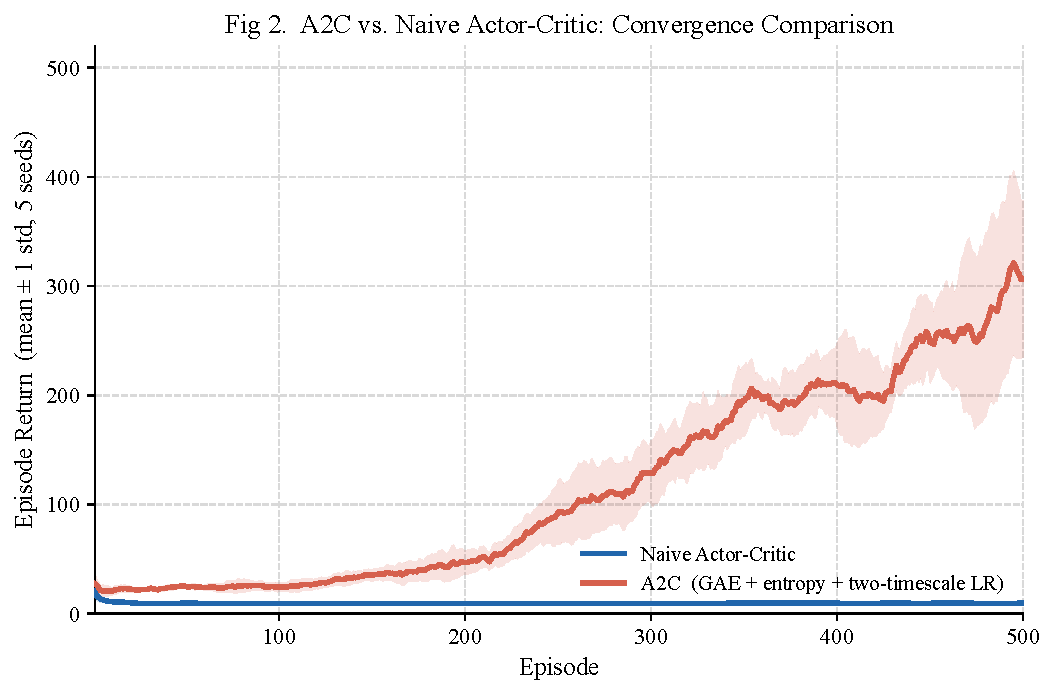
\includegraphics[width=\textwidth]{fig2_a2c_vs_naive.pdf}
  \caption{A2C 与朴素 Actor-Critic 在 CartPole-v1 上的收敛对比（5 seeds，mean $\pm$ 1 std，相同网络结构，仅训练方式不同）。}
  \label{fig:compare}
\end{figure}

回顾图~\ref{fig:adv} 的 A2C 曲线（红色钟形）：前 $\sim 280$ 轮优势信号持续增大，对应 Fig~\ref{fig:compare} 中收益快速上升的阶段——策略改进速度 $>$ Critic 追赶速度；之后随 Critic 追上而平滑回落，收益曲线斜率也随之减缓。\textbf{Critic 与 Actor 的「追赶」动态，正是两时间尺度设计想要保持的健康状态。}

% ============================================================
\section*{算法对比总结}

\[
\begin{array}{c|c|c|c}
\text{方法} & \text{优势估计} & \text{更新时机} & \text{偏差 / 方差} \\
\hline
\text{REINFORCE} & G_t & \text{回合结束} & \text{低偏差，极高方差} \\
\text{REINFORCE + Baseline} & G_t - V(s_t) & \text{回合结束} & \text{低偏差，高方差（改善）} \\
\text{朴素 AC} & \delta_t & \text{每步在线} & \text{高偏差，低方差（但坍缩）} \\
\text{A2C} & \hat{A}^{\text{GAE}(\gamma,\lambda)} & \text{回合后批量} & \text{$\lambda$ 可调，稳定} \\
\end{array}
\]

\subsection*{为什么 A2C 不直接用 Monte Carlo 回报？}

用纯 MC 回报 $G_t$ 作为 Critic 目标，等同于 REINFORCE with baseline——bootstrap 的方差优势消失，退化为在线 MC 更新。在 CartPole-v1 这样的\textbf{短回合}任务中 MC 尚可用，但在连续控制（关节角度、速度等高维动作空间）$+$ 长回合任务中，$G_t$ 的方差会大到无法收敛。GAE 的 $\lambda$ 参数提供了偏差--方差的连续插值，而不必在两个极端中二选一。

\subsection*{为什么 Critic 学习率要高于 Actor？}

\textbf{两时间尺度定理}（Konda \& Tsitsiklis 2003）：Actor-Critic 收敛需满足：

\[
\sum_k \alpha_\theta(k) = \infty, \quad \sum_k \alpha_w(k) = \infty, \quad
\frac{\alpha_\theta(k)}{\alpha_w(k)} \to 0 \quad (k \to \infty)
\]

\textbf{直觉}：如果 Actor 和 Critic 以相同速度变化，Critic 永远在追移动靶（策略一直在变）；
Critic 学得更快，就能在 Actor 下次更新前先近似收敛到当前策略的 $V^\pi$，保证 Actor 拿到的是「对当前策略的准确评估」，梯度方向可信。

% ============================================================
\section*{本章在 RL 体系中的位置}

Actor-Critic 是从基础算法迈向现代深度 RL 的关键桥梁：

\begin{enumerate}
  \item \textbf{TD 路线（基于值）}：MAB $\to$ MDP / Bellman 方程 $\to$ TD(0) / Q-Learning $\to$ DQN。
        DQN 学的是 $Q(s,a)$，是纯 Critic，没有显式 Actor；无法处理连续动作空间。

  \item \textbf{MC 路线（基于策略）}：REINFORCE 直接优化 $\pi_\theta$，是纯 Actor，没有 Critic；
        方差极大，样本效率低。

  \item \textbf{Actor-Critic 路线（融合）}：本章将两条路线合并——Actor 优化策略，Critic 提供低方差基准。
        GAE 控制偏差--方差权衡 $\to$
        \textbf{PPO}（下一章）在 AC 框架上加 clip 约束，限制每步策略更新幅度，避免步长过大破坏已有策略 $\to$
        \textbf{SAC} 在最大熵框架下自动调节温度系数 $\beta$，将熵正则化推向更严格的理论基础。

  \item \textbf{离线 RL 的影子}：IQL（Implicit Q-Learning）等离线方法中，Critic 仍然需要准确的价值估计；
        两时间尺度原则以不同形式复现——\underline{如何在数据集覆盖不足时让 Critic 不过拟合超出分布的状态}，
        正是离线 RL 要回答的核心问题。
\end{enumerate}

把 PPO 的 clip 目标去掉，只保留 GAE + 熵 + 梯度裁剪，你得到的和本章 A2C 有多大区别——PPO 的 clip 究竟防止了什么？

\subsection*{参考资料}

\begin{enumerate}
  \item Konda \& Tsitsiklis (2003). On actor-critic algorithms. \textit{SIAM Journal on Control and Optimization}, 42(4).
  \item Sutton \& Barto (2018). \textit{Reinforcement Learning: An Introduction} (2nd ed.). Chapter 13.
  \item Schulman et al.\ (2015). High-dimensional continuous control using generalized advantage estimation. \textit{ICLR 2016}.
  \item Mnih et al.\ (2016). Asynchronous methods for deep reinforcement learning (A3C). \textit{ICML}.
  \item 动手学强化学习（Hands-on-RL）. 第12章：Actor-Critic 算法.
\end{enumerate}

\end{document}
